\documentclass[12pt,a4paper,oneside]{article}
\usepackage{graphicx,setspace,float,fancyhdr,listings,xcolor,placeins,xeCJK,tocloft,enumerate,amsmath,amssymb,bm}
\usepackage[dvipsnames]{xcolor}
\renewcommand{\cftsecleader}{\cftdotfill{\cftdotsep}} % Enable dot leaders in TOC
\renewcommand{\cftdotsep}{1} % Adjust dot spacing

\date{\Large 2024.11.21}
\author{陈海弘}

\setCJKmainfont[AutoFakeBold=3]{STFangsong} % CJK Font Setup
\setcounter{tocdepth}{3} % Set TOC depth
\setstretch{1.25} % Line spacing

% Page header and footer setup
\setlength{\headheight}{13.6pt}
\addtolength{\topmargin}{-1.6pt}
\pagestyle{fancy}
\fancyhf{}
\fancyhead[C]{\small Machine Learning} % Center header
\fancyfoot[C]{\small \thepage} % Center footer

% Code highlighting setup
\lstset{
    language=Python,
    basicstyle=\ttfamily\small,
    keywordstyle=\bfseries\color{NavyBlue},
    commentstyle=\itshape\color{red!50!green!50!blue!50},
    stringstyle=\bfseries\color{PineGreen!90!black},
    emph={self}, 
    emphstyle=\bfseries\color{Rhodamine},
    backgroundcolor=\color{black!3},
    frame=shadowbox,
    frameround=fttt,
    numbers=left,
    numberstyle=\tiny,
    stepnumber=1,
    numbersep=5pt,
    breaklines=true,
    columns=flexible,
    xleftmargin=1em,
    xrightmargin=-2em,
    aboveskip=1em,
    framexleftmargin=2em,
    escapeinside=``,
}

% Title setup
\title{
    \vspace*{-2cm}
    
\includegraphics[width=0.8\textwidth]{SYSULogo.pdf} \\[1em]
    \vfill
    \LARGE \textbf{机器学习实验报告5} \\[1em]
    \Large
    \begin{tabular}{rl}
        \textbf{姓名:} & \textbf{陈海弘} \\
        \textbf{学号:} & \textbf{23354049}
    \end{tabular}
    \vfill
}

\begin{document}
\maketitle
\newpage
\tableofcontents
\newpage
\section{摘要}
\qquad 本次实验引入的库有:\texttt{numpy, pandas, cvxopt, matplotlib}。实验内容包括线性可分支持向量机与硬间隔最大化、线性支持向量机与软间隔最大化、非线性支持向量机与核函数。实验目的是通过求解对偶问题,得到最优解$\bm{\alpha}^*$,并计算$\bm{\omega}^*$和$b^*$,最后绘制散点图与决策边界。
\section{线性可分支持向量机与硬间隔最大化}
\subsection{数据读入}
\qquad 读入数据集'dataset1.csv',把数据类型都转换成np.double类型,并画出数据集的散点图,给正样本(y为+1)和负样本(y为-1)分别标上不���的颜色。
\begin{lstlisting}
data = pd.read_csv('dataset1.csv')
data = data.astype(np.double)  
X = data.iloc[:, :-1].values  
y = data.iloc[:, -1].values 
plt.figure(figsize=(8, 6))
positive_samples = X[y == 1]  
negative_samples = X[y == -1] 
plt.scatter(positive_samples[:, 0], positive_samples[:, 1], color='blue', label='Positive (+1)', marker='o')
plt.scatter(negative_samples[:, 0], negative_samples[:, 1], color='red', label='Negative (-1)', marker='x')
plt.xlabel('Feature 1')
plt.ylabel('Feature 2')
plt.title('Scatter Plot of Dataset')
plt.legend()
plt.grid()
plt.show()
\end{lstlisting}

\begin{figure}[H]
    \centering
    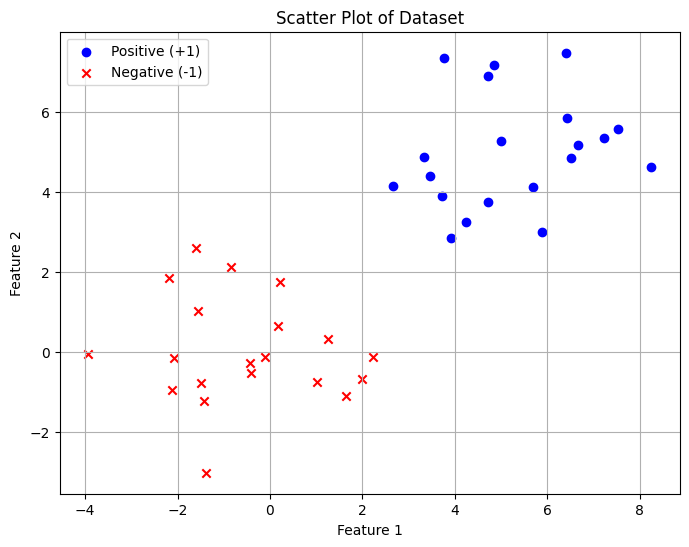
\includegraphics[width=0.8\textwidth]{image/1.png}
    \caption{数据集散点图}
\end{figure}
\subsection{对偶问题求解}
\qquad 求解如下对偶问题:
\[
\begin{aligned}
\min_\alpha \quad & \frac{1}{2}\sum_{i=1}^m\sum_{j=1}^m \alpha_i \alpha_j y_i y_j \bm{x}_i^T \bm{x}_j - \sum_{i=1}^m \alpha_i, \\
\text{s.t.} \quad & \sum_{i=1}^m \alpha_i y_i = 0, \\
& \bm{\alpha} \geq \bm{0}.
\end{aligned}
\]

这个优化问题是一个二次规划问题,其中参数定义如下:
\begin{itemize}
    \item $P$ 是一个 $m \times m$ 的矩阵,其中 $P_{ij} = y_i y_j \bm{x}_i^T \bm{x}_j$,
    \item $q$ 是一个 $m \times 1$ 的列向量,所有值均为 $-1$,即 
    \[
    q := \begin{bmatrix}
    -1 & -1 & \cdots & -1
    \end{bmatrix}^T,
    \]
    \item $G := \begin{bmatrix}
    -1 & 0 & \cdots & 0 \\
    0 & -1 & \cdots & 0 \\
    \vdots & \vdots & \ddots & 0 \\
    0 & 0 & 0 & -1
    \end{bmatrix}_{m \times m} = -\bm{I}, \quad \bm{I} \text{ 为单位矩阵,}$
    \item $h$ 是一个 $m \times 1$ 的零向量,即 
    \[
    h := \begin{bmatrix}
    0 & 0 & \cdots & 0
    \end{bmatrix}^T,
    \]
    \item $A := \begin{bmatrix}
    y_1 & y_2 & \cdots & y_m
    \end{bmatrix}^T, \quad b := \begin{bmatrix} 0 \end{bmatrix} \text{(一个标量)。}$
\end{itemize}

将上述参数送入求解器 \texttt{solvers.qp()} 中即可得到最优解 $\alpha^*$。

\subsection*{附:$P$ 矩阵的计算方法}

设
\[
X = \begin{bmatrix}
x_{11} & x_{12} \\
x_{21} & x_{22} \\
\vdots & \vdots \\
x_{m1} & x_{m2}
\end{bmatrix}, \quad
Y = \begin{bmatrix}
y_1 \\
y_2 \\
\vdots \\
y_m
\end{bmatrix},
\]
计算
\[
X' = \begin{bmatrix}
x_{11} y_1 & x_{12} y_1 \\
x_{21} y_2 & x_{22} y_2 \\
\vdots & \vdots \\
x_{m1} y_m & x_{m2} y_m
\end{bmatrix} = X * Y \quad \text{(注意这里是星乘)},
\]
则 $P = X' {X'}^T$。


本实验的目标是通过求解对偶问题,��到最优解 $\bm{\alpha}^*$。我们利用 \texttt{cvxopt.solvers.qp()} 求解器完成优化,以下为具体实现思路:

\subsection*{1. 数据与参数初始化}
\begin{itemize}
    \item 输入数据 $X$ 的维度为 $m \times n$,其中 $m$ 表示样本数,$n$ 表示特征维数。
    \item 标签向量 $y$ 被重塑为列向量形式,即 $\bm{y} \in \mathbb{R}^m$。
\end{itemize}

\subsection*{2. 构造矩阵 $P$}
\begin{itemize}
    \item 根据公式计算 $X'$:  
    \[
    X' = X * \bm{y},
    \]
    其中 $*$ 表示逐元素相乘(广播操作)。
    \item 计算矩阵 $P$ 为:
    \[
    P = X' {X'}^T.
    \]
    矩阵 $P$ 是目标函数中二次项系数矩阵。
\end{itemize}

\subsection*{3. 定义其他参数}
\begin{itemize}
    \item $q$ 是一个长度为 $m$ 的列向量,所有元素均为 $-1$:
    \[
    q = \begin{bmatrix} -1 \\ -1 \\ \vdots \\ -1 \end{bmatrix}.
    \]
    \item $G$ 是一个 $m \times m$ 的对角矩阵,等于负单位矩阵:
    \[
    G = -\bm{I}.
    \]
    \item $h$ 是一个长度为 $m$ 的零向量:
    \[
    h = \begin{bmatrix} 0 \\ 0 \\ \vdots \\ 0 \end{bmatrix}.
    \]
    \item $A$ 是标签向量 $\bm{y}$ 的转置:
    \[
    A = \bm{y}^T.
    \]
    \item $b$ 是一��标量,值为 $0$:
    \[
    b = \begin{bmatrix} 0 \end{bmatrix}.
    \]
\end{itemize}

\subsection*{4. 转换为 \texttt{cvxopt} 格式}
\begin{itemize}
    \item 矩阵 $P, q, G, h, A, b$ 被转换为 \texttt{cvxopt} 的专用矩阵格式 \texttt{matrix}。
\end{itemize}

\subsection*{5. 调用优化求解器}
\begin{itemize}
    \item 调用 \texttt{solvers.qp()},输入定义的参数:
    \[
    \texttt{solvers.qp(P, q, G, h, A, b)}
    \]
    \item 如果求解报错,可以在调用时添加参数 \texttt{kktsolver='ldl'} 来避免奇异矩阵问题。
\end{itemize}

\subsection*{6. 解析优化结果}
\begin{itemize}
    \item 求解器返回的结果存储在 \texttt{solution['x']} 中。
    \item 将结果展平成一维向量,即为 $\bm{\alpha}$ 的最优解。
\end{itemize}

\subsection*{7. 输出最优解}
最终,程序输出的 $\bm{\alpha}^*$ 即为对偶问题的最优解,满足约束条件:
\[
\bm{\alpha}^* \geq 0, \quad \sum_{i=1}^m \alpha_i^* y_i = 0.
\]

\begin{figure}[H]
    \centering
    
\includegraphics[width=0.6\textwidth]{image/2.png}
    \caption{对偶问题求解结果}
\end{figure}
\subsection{计算 $\bm{\omega}^*$ 和 $b^*$}


通过求解对偶问题得到最优解 $\bm{\alpha}^*$ 后,可以计算 $\bm{\omega}^*$ 和 $b^*$,具体步骤如下:

\subsection*{1. 计算 $\bm{\omega}^*$}
\[
\bm{\omega}^* = \sum_{i=1}^m \alpha_i^* y_i \bm{x}_i,
\]
其中:
\begin{itemize}
    \item $\bm{\alpha}^* \in \mathbb{R}^m$ 是对偶问题的最优解;
    \item $\bm{y} \in \mathbb{R}^m$ 是样本标签向量;
    \item $\bm{x}_i$ 是样本输入向量。
\end{itemize}

\subsection*{2. 计算 $b^*$}
\[
b^* = y_j - \bm{\omega}^{*T} \bm{x}_j,
\]
其中 $j$ 是 $\bm{\alpha}^*$ 中一个正分量 $\alpha_j^* > 0$ 的下标。

\subsection*{3. 筛选 $\alpha^*$ 的正分量}
由于求解器 \texttt{solvers.qp()} 求得的解是近似解,$\bm{\alpha}^*$ 中很多理论上为 0 的分量可能略大于 0。因此,为筛选出有效的正分量,可以采取以下两种方法:
\begin{itemize}
    \item \textbf{方法 1:设置阈值}  
    将 $\bm{\alpha}^*$ 中小于某一阈值 $\epsilon$ 的分量筛去(例如 $\epsilon = 10^{-6}$),剩下的分量中选取一个正分量对应的下标 $j$ 来计算 $b^*$:
    \[
    \bm{\alpha}_\text{筛选} = \{\alpha_i^* \mid \alpha_i^* > \epsilon\}.
    \]
    \item \textbf{方法 2:取最大分量}  
    直接取 $\bm{\alpha}^*$ 中最大的分量 $\max(\bm{\alpha}^*)$ 对应的下标 $j$ 计算 $b^*$。
\end{itemize}

\subsection*{4. 注意事项}
无论选择哪种方法,都需要确保:
\begin{itemize}
    \item 所选 $\alpha_j^* > 0$;
    \item 使用的下标 $j$ 是有效的(即 $j \in \{1, 2, \dots, m\}$)。
\end{itemize}

\begin{lstlisting}
    threshold = 1e-5
    alpha[alpha < threshold] = 0  
    alpha = alpha.reshape(-1, 1)  
    y = y.reshape(-1, 1)     
    omega = np.sum(alpha * y * X, axis=0)  
    print("Optimal ω*:", omega)
    j = np.argmax(alpha)  
    b = y[j] - np.dot(omega, X[j])  
    print("Optimal b*:", b)
\end{lstlisting}

\begin{figure}[H]
    \centering
    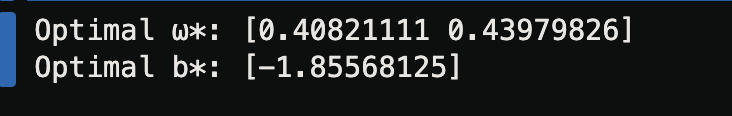
\includegraphics[width=0.6\textwidth]{image/3.png}
    \caption{计算 $\bm{\omega}^*$ 和 $b^*$}
\end{figure}
\subsection{绘制散点图与决策边界}
\qquad 画出数据集的散点图,给正样本($y$为+1)和负样本($y$为-1)分别标上不同的颜色,再为支持向量(训练数据中$\alpha_j^* > 0$的对应的样本)标上不同的颜色,并画出决策边界$\pmb{\omega}^{*T}\pmb{x}+b=0$和间隔边界$\pmb{\omega}^{*T}\pmb{x}+b=1$与$\pmb{\omega}^{*T}\pmb{x}+b=-1$。

\begin{enumerate}
    \item 决策边界 $\pmb{\omega}^{*T}\pmb{x} + b = 0$ 的计算公式为:
    \[
    x_2 = -\frac{\omega_1 \cdot x_1 + b}{\omega_2}.
    \]
    \item 上间隔边界 $\pmb{\omega}^{*T}\pmb{x} + b = 1$ 的计算公式为:
    \[
    x_2 = -\frac{\omega_1 \cdot x_1 + b - 1}{\omega_2}.
    \]
    \item 下间隔边界 $\pmb{\omega}^{*T}\pmb{x} + b = -1$ 的计算公式为:
    \[
    x_2 = -\frac{\omega_1 \cdot x_1 + b + 1}{\omega_2}.
    \]
\end{enumerate}

绘制方法的实现步骤如下:
\begin{enumerate}
    \item 计算特征 $x_1$ 的取值范围:
    \[
    x_{\text{min}} = \min(X[:, 0]) - 1, \quad x_{\text{max}} = \max(X[:, 0]) + 1.
    \]
    \item 在该范围内均匀采样若干点,用于计算决策边界和间隔边界:
    \[
    x_{\text{values}} = \text{linspace}(x_{\text{min}}, x_{\text{max}}, 500).
    \]
    \item 使用上述公式计算 $x_2$ 的值。
\end{enumerate}


\begin{lstlisting}[language=Python, caption=计算并绘制决策边界和间隔边界]
# 计算 x_1 的取值范围
x_min, x_max = X[:, 0].min() - 1, X[:, 0].max() + 1
x_values = np.linspace(x_min, x_max, 500)  # 均匀采样

# 计算决策边界和间隔边界
decision_boundary = -(omega[0] * x_values + b) / omega[1]
margin_positive = -(omega[0] * x_values + b - 1) / omega[1]
margin_negative = -(omega[0] * x_values + b + 1) / omega[1]

# 绘图
plt.plot(x_values, decision_boundary, 'k-', label='Decision Boundary')
plt.plot(x_values, margin_positive, 'k--', label='Margin (+1)')
plt.plot(x_values, margin_negative, 'k--', label='Margin (-1)')
plt.legend()
\end{lstlisting}

\begin{figure}[H]
    \centering
    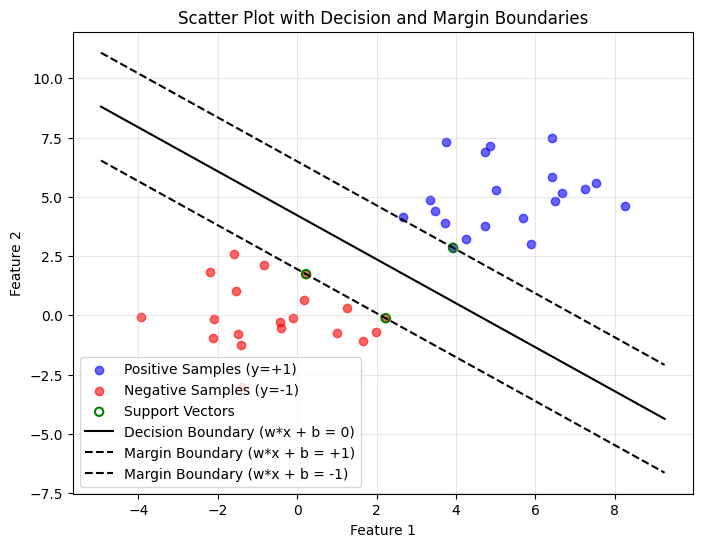
\includegraphics[width=0.8\textwidth]{image/4.png}
    \caption{绘制散点图与决策边界}
\end{figure}

可以看到,红色和蓝色的点被正确分类,且决策边界和间隔边界被正确绘制。
\section{线性支持向量机与软间隔最大化}
\subsection{数据读入}
\begin{lstlisting}
data = pd.read_csv('dataset2.csv')
data = data.astype(np.double)  
print(data.head())
X = data.iloc[:, :-1].values  
y = data.iloc[:, -1].values 
plt.figure(figsize=(8, 6))
positive_samples = X[y == 1]  
negative_samples = X[y == -1] 
plt.scatter(positive_samples[:, 0], positive_samples[:, 1], color='blue', label='Positive (+1)', marker='o')
plt.scatter(negative_samples[:, 0], negative_samples[:, 1], color='red', label='Negative (-1)', marker='x')
plt.xlabel('Feature 1')
plt.ylabel('Feature 2')
plt.title('Scatter Plot of Dataset')
plt.legend()
plt.grid()
plt.show()
\end{lstlisting}
\begin{figure}[H]
    \centering
    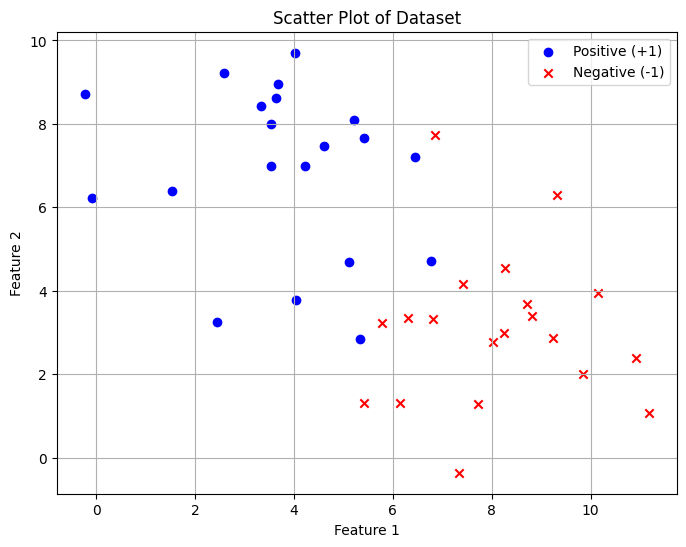
\includegraphics[width=0.8\textwidth]{image/5.png}
    \caption{数据集散点图}
\end{figure}
\subsection{对偶问题求解}

\qquad 硬间隔和软间隔的求解方法相同,只是软间隔在求解时多了一个惩罚系数$C$,这个惩罚系数是用来控制间隔的松弛程度,$C$越大,间隔越小,$C$越小,间隔越大。

支持向量机的目标是通过二次规划(Quadratic Programming, QP)求解优化问题。以下描述了构造二次规划问题的具体步骤:

首先,给定数据集的规模:样本数 $m$ 和特征维度 $n$,分别为:
\[
m = \text{样本数}, \quad n = \text{特征维数}.
\]
定义超参数 $C$,用于控制松弛变量的权重:
\[
C = 7.4.
\]

计算核矩阵 $K$(线性核):
\[
K = X X^T.
\]

构造矩阵 $P$ 和向量 $q$:
\[
P = \text{diag}(y) \cdot K \cdot \text{diag}(y),
\]
\[
q = -\pmb{1}.
\]

构造矩阵 $G$ 和向量 $h$:
\[
G = \begin{bmatrix}
    -\pmb{I} \\
    \pmb{I}
\end{bmatrix}, \quad
h = \begin{bmatrix}
    \pmb{0} \\
    C \cdot \pmb{1}
\end{bmatrix}.
\]

构造矩阵 $A$ 和标量 $b$:
\[
A = \pmb{y}^T, \quad b = 0.
\]

接下来,将上述构造的参数矩阵传入二次规划求解器 \texttt{solvers.qp()},求解问题:
\[
\begin{aligned}
\min_{\pmb{\alpha}} \quad & \frac{1}{2} \pmb{\alpha}^T P \pmb{\alpha} + \pmb{q}^T \pmb{\alpha} \\
\text{s.t.} \quad & G\pmb{\alpha} \preceq h, \\
& A\pmb{\alpha} = b.
\end{aligned}
\]

代码实现如下:
\begin{lstlisting}[language=Python, caption=求解二次规划问题]
# 使用二次规划求解器
sol = solvers.qp(P, q, G, h, A, b)
# 提取结果
alpha = np.array(sol['x']).flatten()
print("Optimal alphas:", alpha)
\end{lstlisting}

通过求解器的输出,可以获得拉格朗日乘子 $\pmb{\alpha}^*$:
\[
\pmb{\alpha}^* = \text{sol['x']}
\]
这些值将用于进一步计算模型参数 $\pmb{\omega}^*$ 和 $b^*$。

\begin{figure}[H]
    \centering
    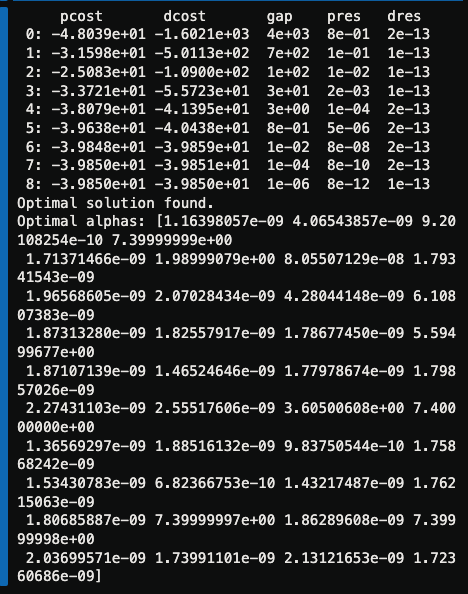
\includegraphics[width=0.6\textwidth]{image/6.png}
    \caption{对偶问题求解结果}
\end{figure}
\subsection{计算 $\bm{\omega}^*$ 和 $b^*$}
在得到优化后的 $\pmb{\alpha}^*$ 后,可以计算支持向量机模型的参数 $\pmb{\omega}^*$ 和偏置项 $b^*$。以下是具体步骤:

1.\textbf{筛选非零 $\pmb{\alpha}^*$}
   因为求解器给出的 $\pmb{\alpha}^*$ 是近似解,有些数值接近 0。我们设置一个阈值 $\text{threshold}$,将所有小于该阈值的 $\pmb{\alpha}$ 置为 0:
   \[
   \text{threshold} = 10^{-5}.
   \]
   过滤后:
   \[
   \pmb{\alpha}^* = 
   \begin{cases} 
   0, & \text{若} \alpha_i^* < \text{threshold}, \\
   \alpha_i^*, & \text{其他}.
   \end{cases}
   \]

2. \textbf{计算 $\pmb{\omega}^*$  }
   模型的权重向量 $\pmb{\omega}^*$ 可通过以下公式计算:
   \[
   \pmb{\omega}^* = \sum_{i=1}^m \alpha_i^* y_i \pmb{x}_i.
   \]

3. \textbf{选择支持向量  }
   从 $\pmb{\alpha}^*$ 中选择一个非零分量 $\alpha_j^* > 0$ 对应的样本索引 $j$。可通过取 $\pmb{\alpha}^*$ 中最大值的下标实现:
   \[
   j = \text{argmax}_i \, \alpha_i^*.
   \]

4.\textbf{ 计算偏置项 $b^*$ } 
   偏置项 $b^*$ 的计算公式为:
   \[
   b^* = y_j - \pmb{\omega}^{*T} \pmb{x}_j,
   \]
   其中,$j$ 为选取的支持向量的下标。

5.\textbf{ 最终结果输出  }
   权重向量 $\pmb{\omega}^*$ 和偏置项 $b^*$ 的值分别为:
   \[
   \pmb{\omega}^* = \text{计算得到的权重向量},
   \]
   \[
   b^* = \text{计算得到的偏置项}.
   \]

以下是代码实现:
\begin{lstlisting}[language=Python, caption=计算 $\omega^*$ 和 $b^*$]
threshold = 1e-5
alpha[alpha < threshold] = 0  
alpha = alpha.reshape(-1, 1)  
y = y.reshape(-1, 1)     
omega = np.sum(alpha * y * X, axis=0)  
print("Optimal ω*:", omega)
j = np.argmax(alpha)  
b = y[j] - np.dot(omega, X[j])  
print("Optimal b*:", b)
\end{lstlisting}

\begin{figure}[H]
    \centering
    
\includegraphics[width=0.6\textwidth]{image/7.png}
    \caption{计算 $\omega^*$ 和 $b^*$}
\end{figure}
\subsection{绘制散点图与决策边界}
画出数据集的散点图,给正样本($y = +1$)和负样本($y = -1$)分别标上不同的颜色,再为支持向量(训练数据中 $\alpha_j^* > 0$ 的对应样本)标上不同的颜色,并画出决策边界 $\bm{\omega}^{*T} \bm{x} + b = 0$ 和间隔边界 $\bm{\omega}^{*T} \bm{x} + b = 1$ 与 $\bm{\omega}^{*T} \bm{x} + b = -1$。
代码实现:
\begin{lstlisting}[language=Python, caption=绘制散点图与决策边界]
    plt.figure(figsize=(8, 6))
    
    support_vectors = X[alpha.flatten() > 1e-5]  
    
    plt.scatter(positive_samples[:, 0], positive_samples[:, 1], color="blue", label="Positive Samples (y=+1)", alpha=0.6)
    plt.scatter(negative_samples[:, 0], negative_samples[:, 1], color="red", label="Negative Samples (y=-1)", alpha=0.6)
    
    plt.scatter(support_vectors[:, 0], support_vectors[:, 1], edgecolors="green", facecolors="none",
                linewidths=1.5, label="Support Vectors")
    
    x_min, x_max = X[:, 0].min() - 1, X[:, 0].max() + 1
    x_values = np.linspace(x_min, x_max, 500)  # 取点
    
    decision_boundary = -(omega[0] * x_values + b) / omega[1]
    margin_positive = -(omega[0] * x_values + b - 1) / omega[1]
    margin_negative = -(omega[0] * x_values + b + 1) / omega[1]
    
    plt.plot(x_values, decision_boundary, "k-", label="Decision Boundary (w*x + b = 0)")
    plt.plot(x_values, margin_positive, "k--", label="Margin Boundary (w*x + b = +1)")
    plt.plot(x_values, margin_negative, "k--", label="Margin Boundary (w*x + b = -1)")
    
    plt.legend()
    plt.title("Scatter Plot with Decision and Margin Boundaries")
    plt.xlabel("Feature 1")
    plt.ylabel("Feature 2")
    plt.grid(alpha=0.3)
    plt.show()
    
\end{lstlisting}

\begin{figure}[H]
    \centering
    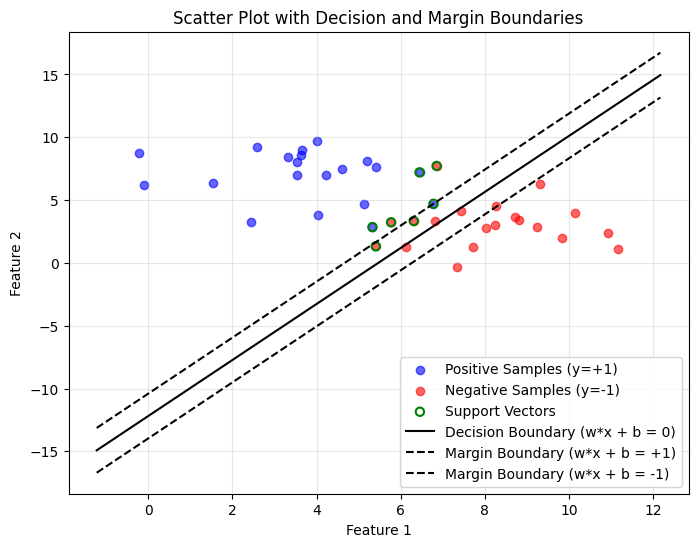
\includegraphics[width=0.8\textwidth]{image/8.png}
    \caption{绘制散点图与决策边界}
\end{figure}
可以看到,蓝点和红点被分类,有些点在决策边界上,有些点在间隔边界上,这些点的颜色不同,支持向量用绿色标出。支持向量可以用来确定决策边界和间隔边界。
\section{非线性支持向量机与核函数}
\subsection{数据读入}
\qquad 
Raisin Dataset是一个葡萄干的数据集,总共有900个样本,每个样本包含7个(都是连续的)特征以及1个标签,每个标签只有两种可能取值。本次实验已经按照8:2的比例划分成了训练数据集'Raisin\_train.csv'以及测试数据集'Raisin\_test.csv',且每个数据集都已经做了特征归一化处理以及把标签的值替换成了+1和-1。
\begin{lstlisting}
    train_data = pd.read_csv('Raisin_train.csv')
    train_data = train_data.astype(np.double)
    print(train_data.dtypes)    
\end{lstlisting}

\subsection{对偶问题求解}
\qquad 选择一个核函数 $K(\bm{x}, \bm{z})$ 以及参数 $C$,求解如下对偶问题(参考课件):
$$
\begin{aligned}
\min_\alpha\quad   &\frac{1}{2}\sum_{i=1}^m\sum_{j=1}^m\alpha_i\alpha_jy_iy_jK(\bm{x}_i, \bm{x}_j)-\sum_{i=1}^m\alpha_i \\
s.t. \quad  &\sum_{i=1}^m\alpha_iy_i=0 \\
      &\bm{0}\leq \bm{\alpha}\leq C 
\end{aligned}
$$

相较于软间隔最大化的优化问题,该优化问题仅需要对矩阵 $P$ 做改动。  
从以下常用的核函数中选择一个作为该优化问题中的 $K$(参数自己进行调整):
- 线性核:$K(\bm{x}, \bm{z}) = \bm{x}^T\bm{z}$
- 多项式核:$K(\bm{x}, \bm{z}) = (\bm{x}^T\bm{z} + 1)^p$
- 高斯核:$K(\bm{x}, \bm{z}) = \exp\left(-\frac{\|\bm{x} - \bm{z}\|^2}{2\sigma^2}\right)$
- 拉普拉斯核:$K(\bm{x}, \bm{z}) = \exp\left(-\frac{\|\bm{x} - \bm{z}\|}{\sigma}\right)$
- Sigmoid核:$K(\bm{x}, \bm{z}) = \tanh(\beta \bm{x}^T\bm{z} + \theta)$

则 $P$ 是一个 $m \times m$ 的矩阵,其中 $P_{ij} = y_i y_j K(\bm{x}_i, \bm{x}_j)$。
\subsection{选择核函数求解对偶问题}

本节展示了使用核方法求解支持向量机(SVM)对偶问题的完整实现流程。代码的主要逻辑分为以下几部分:

\paragraph{Step 1: 构造核矩阵 $K$}
根据输入数据 $\mathbf{X}$ 和标签 $\mathbf{y}$ 计算核矩阵 $K$。支持的核函数包括线性核、多项式核、高斯核(RBF)、拉普拉斯核和 Sigmoid 核:
\begin{itemize}
    \item \textbf{线性核:} $K = \mathbf{X} \mathbf{X}^\top$
    \item \textbf{多项式核:} $K = (\mathbf{X} \mathbf{X}^\top + 1)^p$
    \item \textbf{高斯核 (RBF):} $K_{ij} = \exp\left(-\frac{\|\mathbf{x}_i - \mathbf{x}_j\|^2}{2\sigma^2}\right)$
    \item \textbf{拉普拉斯核:} $K_{ij} = \exp\left(-\frac{\|\mathbf{x}_i - \mathbf{x}_j\|_1}{\sigma}\right)$
    \item \textbf{Sigmoid核:} $K = \tanh(\beta (\mathbf{X} \mathbf{X}^\top) + \theta)$
\end{itemize}
核矩阵通过函数 \texttt{compute\_P} 生成,并根据 $\mathbf{y}$ 构造矩阵 $P$,公式为:
\[
P = \mathbf{y} \mathbf{y}^\top \odot K
\]

\paragraph{Step 2: 对偶问题的优化目标}
SVM 对偶问题的优化目标为:
\[
\max_{\boldsymbol{\alpha}} \quad \frac{1}{2} \boldsymbol{\alpha}^\top P \boldsymbol{\alpha} - \mathbf{1}^\top \boldsymbol{\alpha}
\]
约束条件为:
\[
\begin{aligned}
    &0 \leq \alpha_i \leq C, \quad \forall i \\
    &\mathbf{y}^\top \boldsymbol{\alpha} = 0
\end{aligned}
\]

\paragraph{Step 3: 转换为 \texttt{cvxopt} 格式并求解}
使用 \texttt{cvxopt} 库求解该二次优化问题,具体转换格式如下:
\begin{itemize}
    \item 优化变量 $\boldsymbol{\alpha}$ 的系数矩阵为 $P$
    \item 常数项向量为 $\mathbf{q} = -\mathbf{1}$
    \item 不等式约束矩阵为:
    \[
    \mathbf{G} = \begin{bmatrix}
    -\mathbf{I} \\ 
    \mathbf{I}
    \end{bmatrix}, \quad
    \mathbf{h} = \begin{bmatrix}
    \mathbf{0} \\ 
    C \cdot \mathbf{1}
    \end{bmatrix}
    \]
    \item 等式约束为:
    \[
    \mathbf{A} = \mathbf{y}^\top, \quad b = 0
    \]
\end{itemize}

\paragraph{Step 4: 求解对偶问题}
调用 \texttt{cvxopt.solvers.qp} 求解优化问题,得到优化变量 $\boldsymbol{\alpha}$ 的值。

\paragraph{Step 5: 实现与运行}
最后,根据输入数据 $\mathbf{X}_{\text{train}}$ 和标签 $\mathbf{y}_{\text{train}}$,设置核函数类型与参数(如 $C=1.0$ 和 $\sigma=1.0$),并调用上述步骤完成对 SVM 对偶问题的求解。

我选择的是高斯核函数,和其他核函数一样,高斯核函数的参数 $\sigma$ 也需要调整,这里我选择了 $\sigma=1.0$,并且设置了惩罚系数 $C=1.0$。
代码如下:
\begin{lstlisting}
    def compute_P(X, y, kernel='rbf', kwargs):
    m = X.shape[0]
    y = y.reshape(-1, 1)  # 确保 y 是列向量
        kernel == 'rbf':
        sigma = kwargs.get('sigma', 1.0)
        pairwise_dists = cdist(X, X, 'sqeuclidean')  # 欧氏距离的平方
        K = np.exp(-pairwise_dists / (2 * sigma  2))  # 高斯核
    P = y * y.T * K# 构造 P 矩阵
    return P
    def solve_dual_problem(P, y, C):
        m = P.shape[0]
        # 转换为 cvxopt 格式
        P = matrix(P)
        q = matrix(-np.ones((m, 1)))
        G = matrix(np.vstack((-np.eye(m), np.eye(m))))
        h = matrix(np.hstack((np.zeros(m), C * np.ones(m))))
        A = matrix(y.reshape(1, -1))
        b = matrix(0.0)

        sol = solvers.qp(P, q, G, h, A, b)
        alpha = np.array(sol['x']).flatten()
        return alpha
X_train = train_data.iloc[:, :-1].to_numpy()  # 特征
y_train = train_data.iloc[:, -1].to_numpy()  # 标签

# 转换标签为列向量
y_train = y_train.astype(np.double)

# 参数设置
C = 1.0
sigma = 1.0

# 构造 P
P = compute_P(X_train, y_train, kernel='rbf', sigma=sigma)

# 求解对偶问题
alpha = solve_dual_problem(P, y_train, C)

# 输出结果
print("Optimal alpha values:", alpha)
    \end{lstlisting}

\begin{figure}[H]
    \centering
    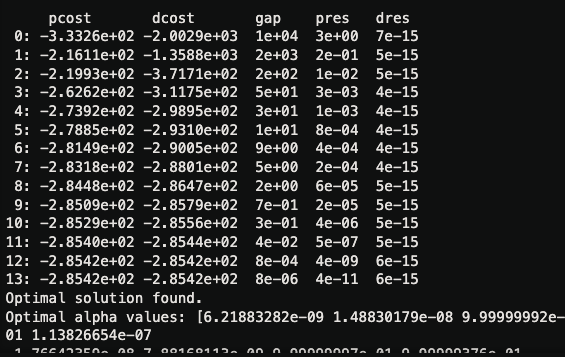
\includegraphics[width=0.6\textwidth]{image/9.png}
    \caption{对偶问题求解结果}
\end{figure}
\subsection{b的计算}
\qquad 1. \textbf{寻找支持向量:}  
   支持向量满足条件 \( 0 < \alpha_i < C \),其中 \( \alpha_i \) 是拉格朗日乘子,\( C \) 是松弛变量的上限。
   \[
   \text{support\_indices} = \{ i \mid \epsilon < \alpha_i < C \}
   \]
   其中 \(\epsilon = 10^{-5}\) 用于数值精度控制。  

   如果未找到支持向量,则报错:  
   \[
   \text{Error: No support vectors found. Check } \alpha \text{ and } C \text{ values.}
   \]

2. \textbf{选择支持向量的一个下标:}  
   选择第一个支持向量 \( j \) 的下标:  
   \[
   j = \text{support\_indices}[0]
   \]  
   对应的支持向量为:  
   \[
   \pmb{x}_j, \, y_j
   \]

3. \textbf{核函数计算 \( K(\pmb{x}_i, \pmb{x}_j) \):}  
   根据核函数类型计算核矩阵 \( K \):  

   - \textbf{线性核(Linear Kernel)  }
     \[
     K(\pmb{x}_i, \pmb{x}_j) = \pmb{x}_i \cdot \pmb{x}_j^T
     \]

   - \textbf{多项式核(Polynomial Kernel) } 
     \[
     K(\pmb{x}_i, \pmb{x}_j) = (\pmb{x}_i \cdot \pmb{x}_j^T + 1)^p
     \]
     其中 \( p \) 为多项式阶数。

   - \textbf{高斯核(RBF Kernel)  }
     \[
     K(\pmb{x}_i, \pmb{x}_j) = \exp\left(-\frac{\|\pmb{x}_i - \pmb{x}_j\|^2}{2\sigma^2}\right)
     \]
     其中 \( \sigma \) 为核函数的参数。

   - \textbf{拉普拉斯核(Laplacian Kernel)  }
     \[
     K(\pmb{x}_i, \pmb{x}_j) = \exp\left(-\frac{\|\pmb{x}_i - \pmb{x}_j\|_1}{\sigma}\right)
     \]

   - Sigmoid Kernel  
     \[
     K(\pmb{x}_i, \pmb{x}_j) = \tanh(\beta \cdot (\pmb{x}_i \cdot \pmb{x}_j^T) + \theta)
     \]
     其中 \( \beta \) 和 \( \theta \) 是核函数的超参数���

   - 如果核类型未知,则报错:  
     \[
     \text{Error: Unknown kernel type.}
     \]

4. \textbf{计算 \( b^* \):}  
   使用公式:  
   \[
   b^* = y_j - \sum_{i=1}^m \alpha_i y_i K(\pmb{x}_i, \pmb{x}_j)
   \]
   其中 \( m \) 是样本数量,\( K(\pmb{x}_i, \pmb{x}_j) \) 是核函数计算结果。


在这里,我选择了高斯核进行计算,惩罚参数和核函数参数与上面一致。
代码如下:
\begin{lstlisting}
    def compute_b_star(X, y, alpha, kernel='rbf', kwargs):
 
    # 找到支持向量:满足 0 < alpha_i < C
    C = kwargs.get('C', 1.0)
    support_indices = np.where((alpha > 1e-5) & (alpha < C))[0]  # 支持向量下标

    # 如果没有支持向量,返回错误提示
    if len(support_indices) == 0:
        raise ValueError("No support vectors found. Check alpha and C values.")
    
    # 使用第一个支持向量的下标
    j = support_indices[0]
    x_j, y_j = X[j], y[j]
    m = X.shape[0]
    kernel == 'rbf':
    sigma = kwargs.get('sigma', 1.0)
    pairwise_dists = np.linalg.norm(X - x_j, axis=1)  2
    K = np.exp(-pairwise_dists / (2 * sigma  2))
    # 计算 b*
    b_star = y_j - np.sum(alpha * y * K)
    return b_star

# 参数设置
C = 1.0
sigma = 1.0

# 计算 b*
b_star = compute_b_star(X_train, y_train, alpha, kernel='rbf', sigma=sigma, C=C)

print(f"Optimal b*: {b_star}")
\end{lstlisting}

\subsection{预测准确率计算}
\qquad 给定测试数据集 \texttt{Raisin\_test.csv},使用分类决策函数对其进行预测,并计算预测准确率。具体步骤如下:

1.\textbf {读入测试数据集:}  
   从文件 \texttt{Raisin\_test.csv} 中读取测试数据集,记为 \(\pmb{x}\)。

2.\textbf {分类决策函数:}  
   对于每个测试样本,使用以下分类决策函数 \( f(\pmb{x}) \) 进行预测:
   \[
   f(\pmb{x}) = \text{sign} \left( \sum_{i=1}^m \alpha_i^* y_i K(\pmb{x}_i, \pmb{x}) + b^* \right)
   \]
   其中:
   \begin{itemize}
       \item \( m \):训练集样本数量;
       \item \( \alpha_i^* \):训练集中的拉格朗日乘子;
       \item \( y_i \):训练集样本的标签;
       \item \( \pmb{x}_i \):训练集样本的特征;
       \item \( \pmb{x} \):测试集样本的特征;
       \item \( K(\pmb{x}_i, \pmb{x}) \):训练样本和测试样本之间的核函数;
       \item \( b^* \):通过支持向量计算得到的偏置。
   \end{itemize}

3. \textbf{计算预测准确率:  }
   将模型预测结果与测试集的真实标签 \( y_{\text{test}} \) 进行比较,计算预测准确率:
   \[
   \text{Accuracy} = \frac{\text{Number of correct predictions}}{\text{Total number of test samples}} \times 100\%
   \]

4.\textbf {输出预测准确率:  }
   将最终的预测准确率以百分比形式输出。

   重要代码如下:
\begin{lstlisting}
    def predict_and_evaluate(X_train, y_train, alpha, b_star, X_test, y_test, kernel='rbf', kwargs):

    m_train = X_train.shape[0]
    m_test = X_test.shape[0]

    elif kernel == 'rbf':
        sigma = kwargs.get('sigma', 1.0)
        pairwise_dists = cdist(X_train, X_test, 'sqeuclidean')  # 欧氏距离的平方
        K = np.exp(-pairwise_dists / (2 * sigma  2))

    # 计算分类决策函数 f(x) = sign(Σ α_i * y_i * K(x_i, x) + b*)
    f_x = np.dot(alpha * y_train, K) + b_star
    y_pred = np.sign(f_x)

    # 计算准确率
    accuracy = np.mean(y_pred == y_test)
    return accuracy

accuracy = predict_and_evaluate(
    X_train=X_train,
    y_train=y_train,
    alpha=alpha,
    b_star=b_star,
    X_test=X_test,
    y_test=y_test,
    kernel='rbf',  # 使用高斯核
    sigma=1.0      # 高斯核参数
)

print(f"Prediction accuracy: {accuracy * 100:.2f}%")
\end{lstlisting}

\begin{figure}[H]
    \centering
    
\includegraphics[width=0.6\textwidth]{image/10.png}
    \caption{预测准确率}
\end{figure}

最后的正确率高达87.22\%,说明高斯核函数对于这个数据集是有效的。
\section{实验总结}
\qquad 这次试验主要是对支持向量机的理论知识进行了实践,通过对线性支持向量机和非线性支持向量机的实现,我对支持向量机的工作原理有了更深入的理解。通过实验,我学会了如何使用 Python 的 \texttt{cvxopt} 库来求解二次规划问题,以及如何使用核函数来处理非线性分类问题。在实验中,我还学会了如何绘制支持向量机的决策边界和间隔边界,以及如何计算支持向量机的预测准确率。总的来说,这次实验让我对支持向量机的原理和实现有了更深入的认识,也提高了我的编程能力和数据分析能力。

硬间隔最大化就是通过最大化间隔来找到最优的决策边界,而软间隔最大化则是通过引入松弛变量来允许一些样本点出现在间隔边界和决策边界之间。通过引入惩罚系数 $C$,可以控制间隔的松弛程度,$C$ 越大,间隔越小,$C$ 越小,间隔越大。在实验中,我通过调整 $C$ 的值,观察了支持向量机的决策边界和间隔边界的变化。

这些是线性支持向量机,而非线形支持向量机则是通过核函数来将数据映��到高维空间,从而使数据在高维空间中线性可分。也就是映射到一个平面,然后在平面上找到最优的决策边界。实验中我选择了高斯核函数,通过调整核函数的参数 $\sigma$,观察了支持向量机的预测准确率的变化。通过实验,我对支持向量机的工作原理和实现有了更深入的理解。
\end{document}